\documentclass[11pt,letterpaper]{article}

% ---------- Typography: serif body, sans headings (institutional memo standard) ----------
\usepackage[margin=1.05in,top=0.95in,bottom=1in]{geometry}
\usepackage[T1]{fontenc}
\usepackage{mathpazo}            % Palatino body — the classic finance-document serif
\usepackage{helvet}              % Helvetica for headings and labels only
\usepackage{microtype}           % refined kerning and justification
\usepackage{xcolor}
\usepackage[colorlinks=true,urlcolor=navy,linkcolor=navy]{hyperref}
\urlstyle{sf}                    % URLs in the document's sans font, not monospace
\usepackage{enumitem}
\usepackage{fancyhdr}
\usepackage{lastpage}
\usepackage{array}
\usepackage{graphicx}

\definecolor{navy}{HTML}{1F3864}
\definecolor{midgray}{HTML}{595959}
\definecolor{hairline}{HTML}{C8C8C8}

\linespread{1.10}                % comfortable executive leading
\setlength{\parindent}{0pt}
\setlength{\parskip}{3.5pt}

% ---------- Footer: understated, informational ----------
\pagestyle{fancy}
\fancyhf{}
\renewcommand{\headrulewidth}{0pt}
\fancyfoot[L]{\sffamily\fontsize{7.5}{9}\selectfont\color{midgray}ENNACIRI \textbar\ PREDICTING U.S. BANK DISTRESS \textbar\ JULY 2026}
\fancyfoot[R]{\sffamily\fontsize{7.5}{9}\selectfont\color{midgray}\thepage\ OF \pageref{LastPage}}

% ---------- Section label: small uppercase bold sans, navy — corporate memo register ----------
\newcommand{\sectionhead}[1]{%
  \vspace{6pt}%
  {\sffamily\bfseries\fontsize{9.5}{12}\selectfont\color{navy}\MakeUppercase{#1}}\par
  \vspace{-9pt}\textcolor{hairline}{\rule{\textwidth}{0.5pt}}\par\vspace{0pt}}

% Answer body
\newcommand{\answer}[1]{#1\par\vspace{3pt}}

\begin{document}

% ---------- Title block ----------
\vspace*{-14pt}
{\sffamily\fontsize{8.5}{11}\selectfont\color{midgray}MSDS 696 DATA SCIENCE PRACTICUM II \quad\textbar\quad WEEK 3 STATUS REPORT}\par\vspace{10pt}
{\sffamily\bfseries\fontsize{21}{25}\selectfont\color{navy}Predicting U.S. Bank Distress}\par\vspace{9pt}
{\sffamily\fontsize{9}{12}\selectfont Oussama Ennaciri \quad\textbar\quad Week 3 \quad\textbar\quad July 19, 2026}\par\vspace{5pt}
\textcolor{navy}{\rule{\textwidth}{1.2pt}}

% ---------- Project title ----------
\sectionhead{Project title}
\answer{Predicting U.S.\ Bank Distress}

% ---------- Project summary ----------
\sectionhead{Project summary}
\answer{This project builds an early-warning model that uses public FDIC and FRED quarterly data to flag which U.S.\ banks are at risk of becoming undercapitalized. The data consists of five linked FDIC tables (1.68M bank-quarter records of each bank's quarterly financial and regulatory filings) plus a FRED macro table (economic context like interest rates, unemployment, and GDP). Data understanding is complete; the next step is feature selection and preparing the data for modeling.}

% ---------- Milestones ----------
\sectionhead{Milestones}
\answer{\begin{enumerate}[topsep=1pt,itemsep=1pt,leftmargin=16pt,label=\textcolor{navy}{\bfseries\arabic*.}]
  \item Literature review of bank failure and existing early-warning models (\textit{in progress})
  \item Collect the data (FDIC API, 1984 to present) (\textbf{DONE})
  \item Understand the data through exploratory data analysis (\textbf{DONE})
  \item Prepare the data for machine learning (\textit{Next})
  \item Train and compare three candidate models
\end{enumerate}}

% ---------- Last week's To Do ----------
\sectionhead{Last week's ``To Do''}
\answer{From the Week 2 report:
\begin{enumerate}[topsep=1pt,itemsep=1pt,leftmargin=16pt,label=\textcolor{navy}{\bfseries\arabic*.}]
  \item Continuing the literature review (\textbf{in progress})
  \item Understanding the data to do feature selection (\textbf{DONE})
\end{enumerate}}

% ---------- This week's progress ----------
\sectionhead{This week's progress}
\answer{Completed the data-understanding phase. Consolidated the literature into a features list per dataset, and verified the exact regulatory definitions behind the target label (becoming undercapitalized) against the regulations (12 CFR 324.403 and its predecessors). Built the working modeling table: 1.26M bank-quarter records (1990--2026) joined with bank statics and macro context, with the distress label. The target is rare: 0.73\% of healthy bank-quarters cross into distress within the following year.

The key EDA finding (figure below): banks that later became undercapitalized show visible deterioration across all six core vitals for roughly two years beforehand, while matched healthy banks tracked over the same calendar quarters stay flat. The eventual cases are already measurably weaker two years out. The decline is bank-specific, not only macro-driven.

\begin{center}
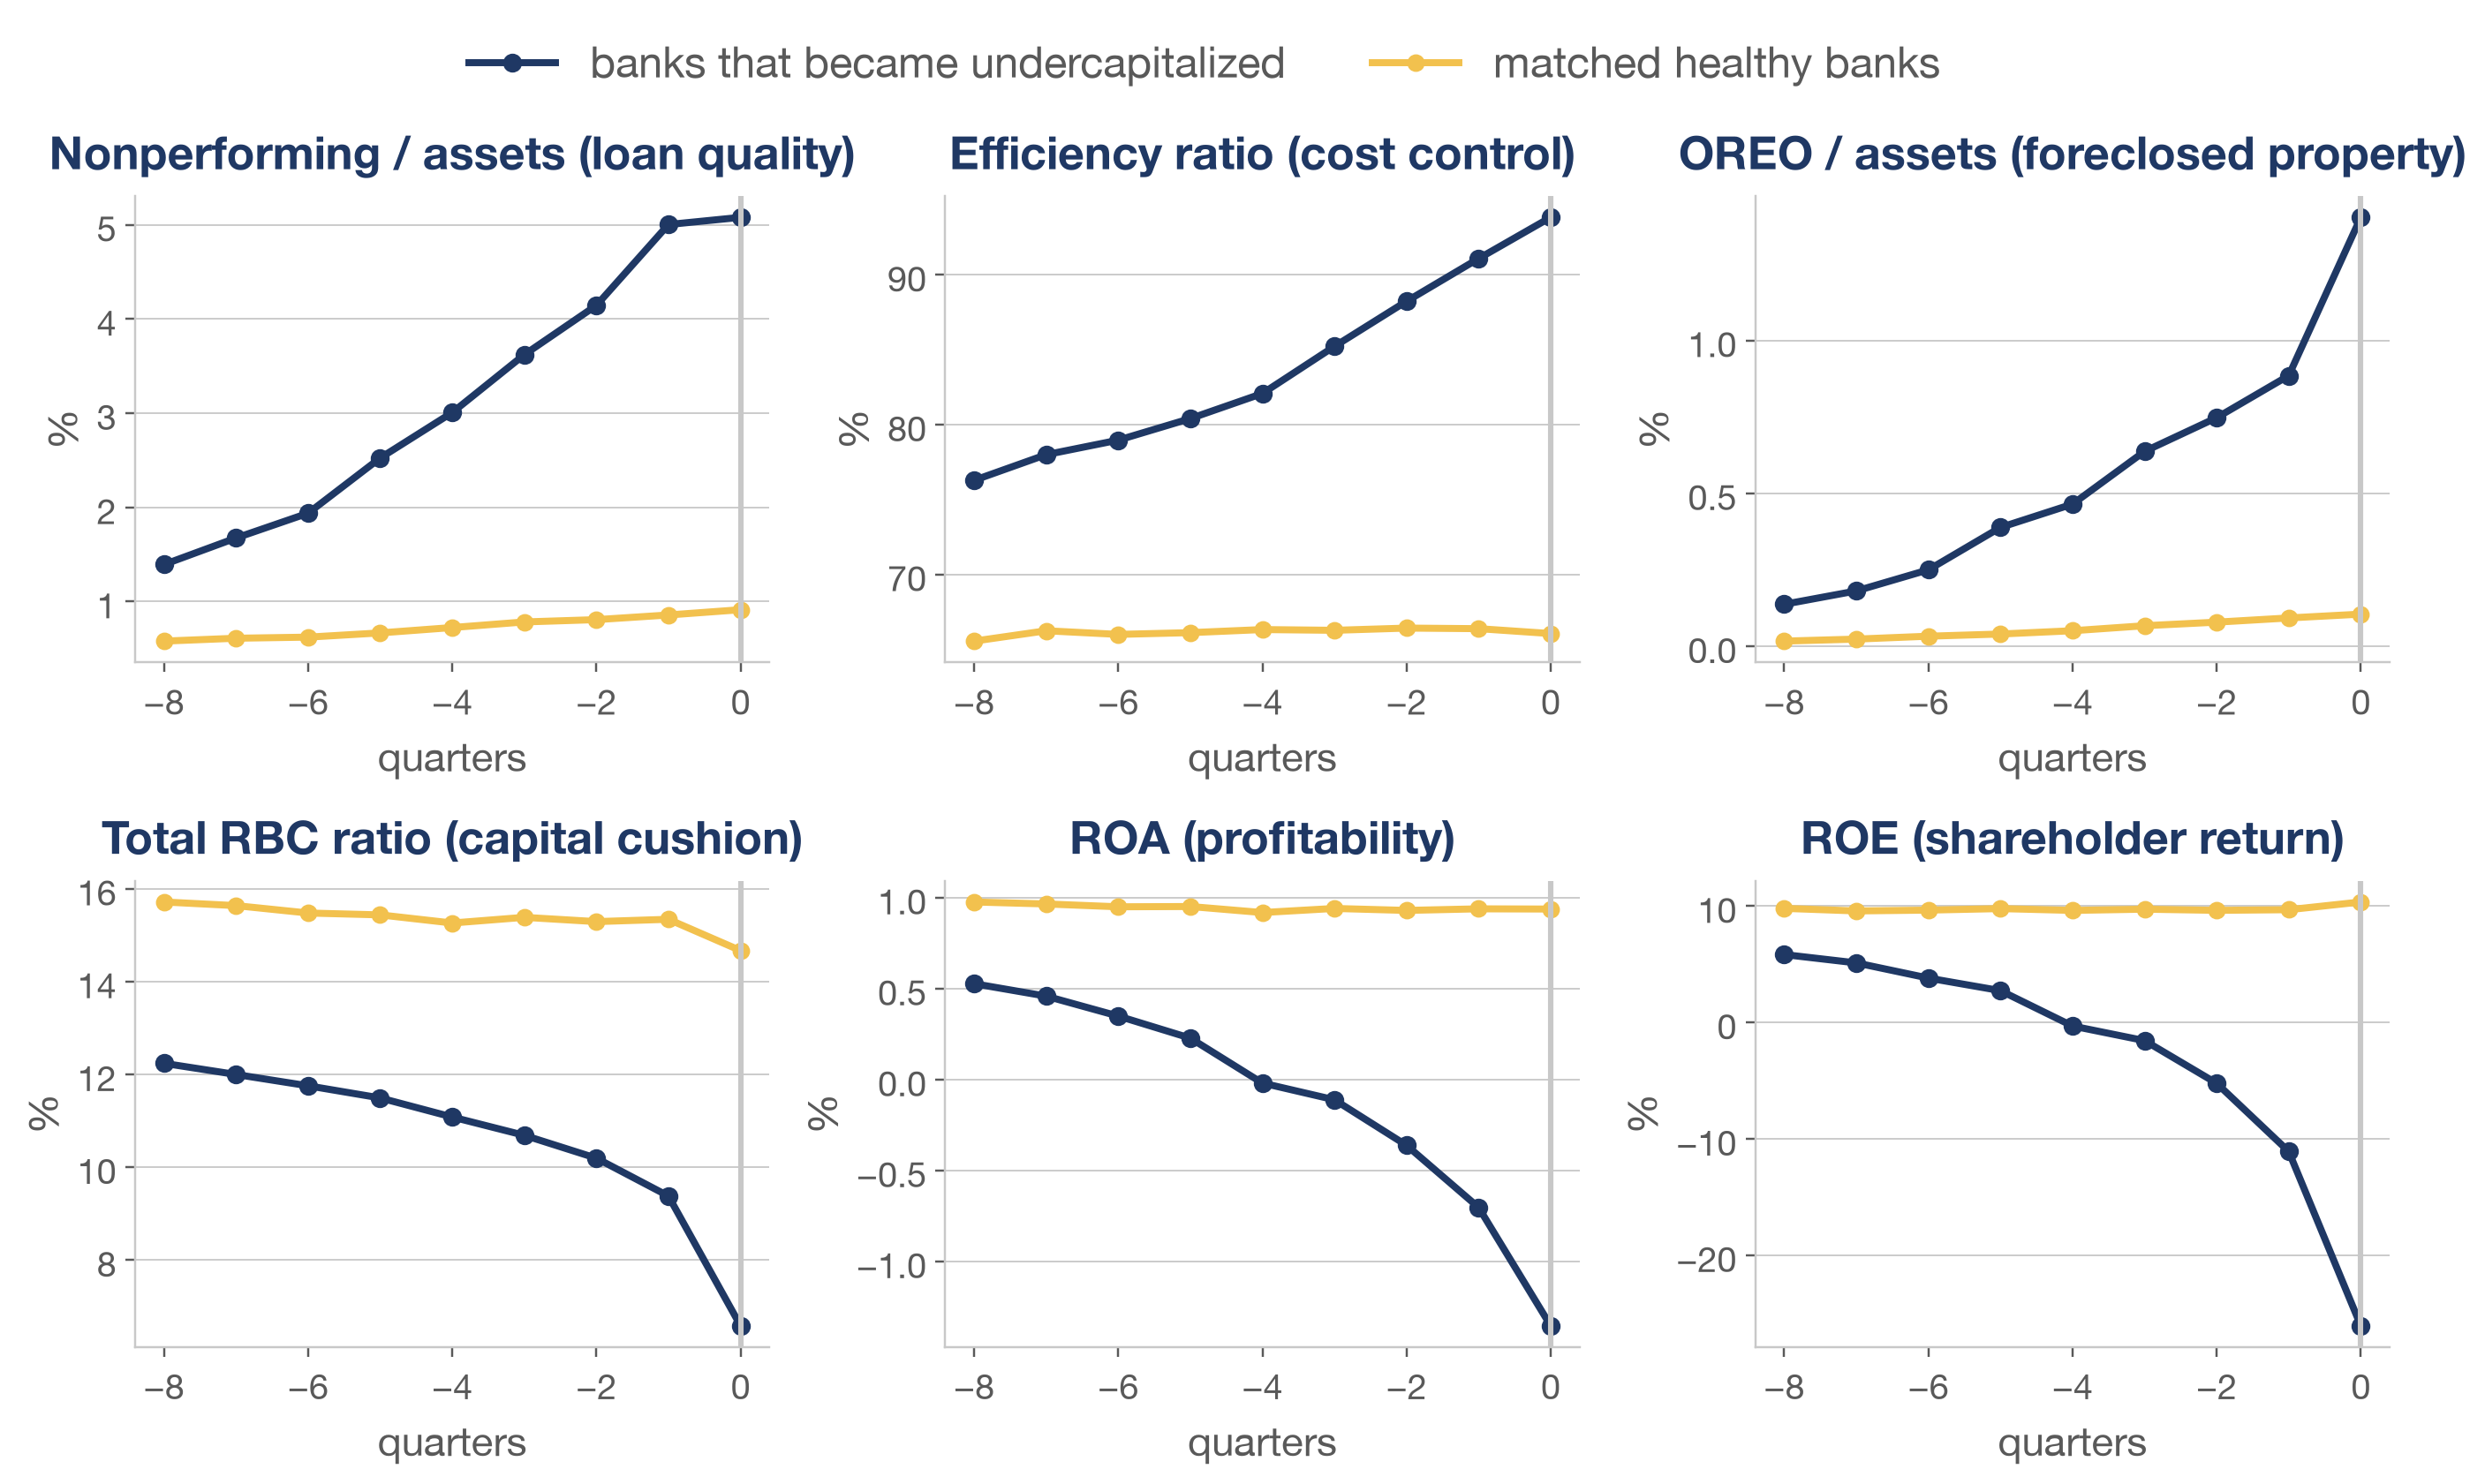
\includegraphics[width=\textwidth]{assets/road_to_trouble.png}
\end{center}
{\fontsize{9}{12}\selectfont\textbf{Figure 1}\par
\textit{Median financial vitals over the eight quarters before a bank became undercapitalized (quarter 0).} Navy: all banks that became undercapitalized, each aligned to its own quarter 0. Gold: healthy banks tracked over the same calendar quarters.\par}}

% ---------- Issues & discussion ----------
\sectionhead{Issues \& discussion}
\answer{\begin{itemize}[topsep=1pt,itemsep=1pt,leftmargin=14pt,label=\textcolor{navy}{\footnotesize\textbullet}]
  \item The target is severely imbalanced: about 7 in 1,000 healthy bank-quarters become undercapitalized within a year. The evaluation metric has to be built around catching the rare cases.
  \item Data leakage is a risk for this problem: the label looks into the future, so training and validation must be split by time, with a gap year, and every feature must use only data available as of the prediction quarter.
  \item Some failures don't follow the two-year decline pattern: SVB's official ratios looked healthy right up to its collapse. Fast, liquidity-driven failures will need funding-stability features beyond the classic ratios.
\end{itemize}}

% ---------- Next week's To Do ----------
\newpage
\sectionhead{Next week's ``To Do''}
\answer{\begin{enumerate}[topsep=1pt,itemsep=1pt,leftmargin=16pt,label=\textcolor{navy}{\bfseries\arabic*.}]
  \item Implement the time-based train/test split
  \item Feature selection: filter pass, then model-based ranking
\end{enumerate}}

% ---------- Resources ----------
\sectionhead{Resources}
\answer{Literature review sources reviewed so far:
\begin{itemize}[topsep=1pt,itemsep=1pt,leftmargin=14pt,label=\textcolor{navy}{\footnotesize\textbullet}]
  \item Cole and White, ``D\'{e}j\`{a} Vu All Over Again: The Causes of U.S.\ Commercial Bank Failures This Time Around,'' \textit{Journal of Financial Services Research}, 2012, Vol.\ 42, No.\ 1, pp.\ 5--29.
  \item Collier, Forbush, Nuxoll, and O'Keefe, ``The SCOR System of Off-Site Monitoring: Its Objectives, Functioning, and Performance,'' \textit{FDIC Banking Review}, 2003, Vol.\ 15, No.\ 3.
  \item Petropoulos, Siakoulis, Stavroulakis, and Vlachogiannakis, ``Predicting Bank Insolvencies Using Machine Learning Techniques,'' \textit{International Journal of Forecasting}, 2020, Vol.\ 36, No.\ 3, pp.\ 1092--1113.
  \item Correia, Luck, and Verner, ``Failing Banks,'' Federal Reserve Bank of New York Staff Report No.\ 1117, September 2024, revised June 2025.
  \item Chu, Frazier, Martin, Agarwal, Kuo, Northwood, Oey, Reed, Rodrigue, and Starr, ``Dissecting Depositor Flight: An Analysis of the Spring 2023 Bank Failures,'' FDIC.
  \item 12 CFR \S\ 324.403, Capital measures and capital category definitions (the PCA thresholds behind the target label).
\end{itemize}}

% ---------- LLM note ----------
\vspace{2pt}
{\small\itshape\color{midgray}\textbf{Note on LLM use:} This document was typeset in LaTeX using Claude Code, which handled the formatting, styling code, and wording polish. All content, research, and decisions are my own, and every suggested edit was reviewed and approved by me.}

\end{document}
